\documentclass[reprint,amsmath,amssymb,aps]{revtex4-2}

\usepackage{graphicx}
\usepackage[caption=false]{subfig}
\usepackage{dcolumn}
\usepackage{bm}
\usepackage{amsmath}
\usepackage{hyperref}
\usepackage{xcolor}
\usepackage{braket}  % Bra-ket notation
\usepackage{float}
\usepackage{tikz}
% \usepackage{subcaption}
% \usepackage{cancel}  % Cancel terms in equations
% \usepackage{caption}
% \usepackage{epsfig}
% \usepackage{rotating}
% \usepackage{enumerate}

\bibliographystyle{apsrev4-2}
\usetikzlibrary{arrows.meta}

\def\iio{{$\langle 110 \rangle$}}
\def\iii{{$\langle 111 \rangle$}}
\def\etal{{\em et al.\/}}

\newcommand{\degree}{\ensuremath{^\circ}}

\definecolor{cblue}{HTML}{607B8F}
\definecolor{cred}{HTML}{9E3B3B}
\definecolor{cred2}{HTML}{EA7B7B}
\definecolor{cgreen}{HTML}{84B179}

\begin{document}

\preprint{APS/123-QED}

\title{Computational Approach to Ultrafast\\Hydrogen Bonding in Water and Ice}

\author{Author(s)}
\date{\today}

\begin{abstract}
	Lorem ipsum dolor sit amet, consectetur adipiscing elit, sed do eiusmod tempor incididunt ut labore et dolore magna aliqua. Ut enim ad minim veniam, quis nostrud exercitation ullamco laboris nisi ut aliquip ex ea commodo consequat. Duis aute irure dolor in reprehenderit in voluptate velit esse cillum dolore eu fugiat nulla pariatur. Excepteur sint occaecat cupidatat non proident, sunt in culpa qui officia deserunt mollit anim id est laborum.
\end{abstract}

\maketitle

\section{Introduction}
% Water is a paradigmatic hydrogen-bonded system whose macroscopic properties emerge from a highly cooperative and continuously fluctuating network of intermolecular interactions. Unlike simple liquids, its local structure is neither rigid nor fully random: directional hydrogen bonds impose transient constraints that couple intermolecular organization to intramolecular vibrations. As a result, structural correlations and molecular motions are deeply intertwined, and even localized perturbations can induce collective responses across the network. This interplay persists across phases, from the disordered liquid to crystalline ices with distinct topologies and degrees of proton order, making water an ideal framework to investigate how vibrational excitations propagate in a correlated molecular environment.\\

Experimentally, ultrafast vibrational spectroscopy has provided detailed insight into the nonequilibrium dynamics of water. Infrared pump–probe measurements have revealed sub-picosecond relaxation of the O–H stretching mode and rapid redistribution of excess energy toward bending and librational modes within the hydrogen-bond network \cite{dettori2019energy}. Complementary two-dimensional infrared (2D-IR) spectroscopy has further established a direct connection between vibrational frequency and local hydrogen-bond configuration, enabling the time-resolved observation of spectral diffusion and hydrogen-bond rearrangements \cite{lspot}. In particular, the evolution of 2D line shapes demonstrates that the O–H stretching frequency reflects instantaneous hydrogen-bond geometry and that structural fluctuations occur on femtosecond to picosecond timescales. While these techniques provide exquisite temporal resolution and indirect structural sensitivity, disentangling vibrational energy redistribution from the underlying microscopic reorganization of the hydrogen-bond network remains challenging.\\

Computationally, atomistic simulations provide direct access to the microscopic pathways underlying vibrational energy relaxation in hydrogen-bonded liquids. On the one hand, equilibrium molecular dynamics combined with mixed quantum–classical frequency mapping schemes has enabled the calculation of infrared and two-dimensional infrared response functions from atomistic trajectories, establishing a quantitative link between vibrational frequency fluctuations and hydrogen-bond rearrangements \cite{roberts2009structural}. In this framework, simulations serve both as an interpretative tool for spectral diffusion and as a benchmark for water models against experimental observables. On the other hand, nonequilibrium molecular dynamics approaches have been developed to mimic pump–probe excitation protocols directly. Methods based on frequency-selective thermostats allow controlled excitation of a targeted vibrational mode while leaving the remaining degrees of freedom near equilibrium, followed by microcanonical evolution to probe energy redistribution pathways. A notable example is the generalized Langevin equation (GLE) approach introduced to simulate vibrational energy relaxation in pump–probe spectroscopy, where a colored-noise “hotspot” thermostat selectively excites a narrow frequency window and subsequent relaxation is monitored in the NVE ensemble \cite{dettori2017simulating}.\\
While these methods provide molecular-level insight into relaxation mechanisms and characteristic time scales, establishing a direct correlation between selective vibrational excitation and the transient structural response of the hydrogen-bond network remains incomplete, particularly across phases with distinct topologies.\\

In this work, we address this challenge by combining selective vibrational excitation with large-scale atomistic simulations of water across distinct phases. We initialize a controlled nonequilibrium state by exciting a fraction of O–H stretching modes using Wigner sampling, followed by microcanonical molecular dynamics evolution with a machine-learned interatomic potential that retains near first-principles accuracy while enabling system sizes sufficient to capture collective network effects. Rather than directly simulating a spectroscopic observable, our approach focuses on the microscopic dynamics of energy redistribution and structural response under controlled excitation conditions. By analyzing time-resolved vibrational densities of states, mode-resolved temperatures, and radial distribution functions, we directly correlate vibrational energy redistribution with the transient structural response of the hydrogen-bond network. Importantly, we perform a systematic comparison between liquid water, proton-disordered ice Ih, and proton-ordered ice IX, thereby disentangling the roles of structural disorder, lattice constraints, and proton ordering in governing ultrafast energy flow. This unified framework provides an atomistic perspective on how network topology and degree of order influence the coupling between localized vibrational excitation and collective hydrogen-bond rearrangements.

Water is a paradigmatic hydrogen-bonded system whose macroscopic properties emerge from a highly cooperative and continuously fluctuating network of intermolecular interactions. Unlike simple liquids, its local structure is neither rigid nor fully random: directional hydrogen bonds impose transient constraints that couple intermolecular organization to intramolecular vibrations. As a result, structural correlations and molecular motions are deeply intertwined, and even localized perturbations can induce collective responses across the network. This interplay persists across phases, from the disordered liquid to crystalline ices with distinct topologies and degrees of proton order, making water an ideal framework to investigate how vibrational excitations propagate in a correlated molecular environment.\\

Experimentally, ultrafast vibrational spectroscopy has provided detailed insight into the nonequilibrium dynamics of water. Infrared pump–probe measurements have revealed sub-picosecond relaxation of the O–H stretching mode and rapid redistribution of excess energy toward bending and librational modes within the hydrogen-bond network \cite{dettori2019energy}. Complementary two-dimensional infrared (2D-IR) spectroscopy has further established a direct connection between vibrational frequency and local hydrogen-bond configuration, enabling the time-resolved observation of spectral diffusion and hydrogen-bond rearrangements \cite{lspot}. In particular, the evolution of 2D line shapes demonstrates that the O–H stretching frequency reflects instantaneous hydrogen-bond geometry and that structural fluctuations occur on femtosecond to picosecond timescales. While these techniques provide exquisite temporal resolution and indirect structural sensitivity, disentangling vibrational energy redistribution from the underlying microscopic reorganization of the hydrogen-bond network remains challenging.\\

Computationally, atomistic simulations provide direct access to the microscopic pathways underlying vibrational energy relaxation in hydrogen-bonded liquids. On the one hand, equilibrium molecular dynamics combined with mixed quantum–classical frequency mapping schemes has enabled the calculation of infrared and two-dimensional infrared response functions from atomistic trajectories, establishing a quantitative link between vibrational frequency fluctuations and hydrogen-bond rearrangements \cite{roberts2009structural}. In this framework, simulations serve both as an interpretative tool for spectral diffusion and as a benchmark for water models against experimental observables. On the other hand, nonequilibrium molecular dynamics approaches have been developed to mimic pump–probe excitation protocols directly. Methods based on frequency-selective thermostats allow controlled excitation of a targeted vibrational mode while leaving the remaining degrees of freedom near equilibrium, followed by microcanonical evolution to probe energy redistribution pathways. A notable example is the generalized Langevin equation (GLE) approach introduced to simulate vibrational energy relaxation in pump–probe spectroscopy, where a colored-noise “hotspot” thermostat selectively excites a narrow frequency window and subsequent relaxation is monitored in the NVE ensemble \cite{dettori2017simulating}.\\
While these methods provide molecular-level insight into relaxation mechanisms and characteristic time scales, establishing a direct correlation between selective vibrational excitation and the transient structural response of the hydrogen-bond network remains incomplete, particularly across phases with distinct topologies.\\

In this work, we address this challenge by combining selective vibrational excitation with large-scale atomistic simulations of water across distinct phases. We initialize a controlled nonequilibrium state by exciting a fraction of O–H stretching modes using Wigner sampling, followed by microcanonical molecular dynamics evolution with a machine-learned interatomic potential that retains near first-principles accuracy while enabling system sizes sufficient to capture collective network effects. Rather than directly simulating a spectroscopic observable, our approach focuses on the microscopic dynamics of energy redistribution and structural response under controlled excitation conditions. By analyzing time-resolved vibrational densities of states, mode-resolved temperatures, and radial distribution functions, we directly correlate vibrational energy redistribution with the transient structural response of the hydrogen-bond network. Importantly, we perform a systematic comparison between liquid water, proton-disordered ice Ih, and proton-ordered ice IX, thereby disentangling the roles of structural disorder, lattice constraints, and proton ordering in governing ultrafast energy flow. This unified framework provides an atomistic perspective on how network topology and degree of order influence the coupling between localized vibrational excitation and collective hydrogen-bond rearrangements.

\begin{figure*}
	\centering
	\subfloat[]{%
		\includegraphics[width=0.33\textwidth]{figures/water.png}
		\label{fig:samples_water}
	}
	\subfloat[]{%
		\includegraphics[width=0.33\textwidth]{figures/iceIh.png}
		\label{fig:samples_iceIh}
	}
	\subfloat[]{%
		\includegraphics[width=0.33\textwidth]{figures/iceIX.png}
		\label{fig:samples_iceIX}
	}
	\caption{
		Representative configurations of the three phases investigated in this work:
		(a) liquid water, (b) proton-disordered ice Ih, and (c) proton-ordered ice IX.
		Liquid water is characterized by a continuously fluctuating and structurally disordered network,
		whereas ice Ih retains a crystalline lattice with orientational proton disorder.
		In contrast, ice IX exhibits a fully proton-ordered structure with a more regular hydrogen-bond arrangement.
	}
	\label{fig:samples}
\end{figure*}


\section{Computational Details}
% \input{sections/Compu}
\subsection{Generation of Equilibrium Samples}
Before investigating the non-equilibrium response induced by vibrational
excitation, we generated equilibrium reference samples for liquid water, ice Ih,
and ice IX using consistent preparation protocols.\\

The liquid water samples were generated from an equilibrium configuration at
ambient temperature, which was replicated to obtain a system of one thousand
molecules (Fig.~\ref{fig:samples_water}). The system was generated inside a cubic cell, whose side length was chosen to reproduce an initial target mass density of $1 \mathrm{g/cm^3}$.\\

In contrast to the liquid phase, the generation of crystalline ice configurations requires explicit control over proton ordering and lattice symmetry, as well as compliance with the Ice Rules. Under these constraints, crystalline ice samples were generated using the GenIce framework \cite{GenIce}.\\
In order to account for different proton orderings, we chose to represent two
ice phases: the Ih phase (Fig.~\ref{fig:samples_iceIh}), which is the stable
proton-disordered form of ice under ambient-pressure conditions, and the IX
(Fig.~\ref{fig:samples_iceIX}) phase, which corresponds to a proton-ordered crystalline structure. For ice Ih, GenIce was used to generate configurations satisfying the ice rules with disordered proton arrangements consistent with the Ih lattice symmetry. For ice IX, a proton-ordered configuration consistent with the corresponding crystallographic structure was generated, without the need for averaging over multiple proton disorder realizations.\\

Due to the constraints imposed by the GenIce framework on the construction of periodic crystalline cells, the ice Ih and ice IX unit cells were replicated to obtain supercells containing 3072 and 2880 atoms, respectively. These system sizes were chosen as the closest multiples compatible with the underlying lattice symmetries and comparable to the system size used for liquid water.


\subsection{Interaction Model and Computational Framework}
All molecular dynamics simulations in this study were performed using a neural network interatomic potential of the NEP (Neuro-Evolution Potential) class. The NEP framework represents the total energy of the system as a sum of atomic contributions expressed as functions of the local environment, with parameters trained on density functional theory (DFT) reference data. This class of potentials has been shown to provide near first-principles accuracy while retaining the computational efficiency required for large-scale molecular dynamics simulations, and has been validated for both liquid water and crystalline ice phases \cite{nep}. The simulations were carried out using the GPUMD package, which provides a native implementation of NEP potentials and enables efficient GPU-accelerated molecular dynamics. All equilibrium and non-equilibrium trajectories discussed in this work were generated within this computational framework.



\subsection{Simulation Protocol}
For each system, an equilibration stage was first performed to ensure thermodynamic stability prior to the excitation procedure. Equilibration was carried out in the isothermal–isobaric (NPT) ensemble. The temperature was controlled using a Nosé–Hoover chain thermostat, while pressure was regulated through a Berendsen barostat, allowing the simulation cell to relax to the target density. Liquid water was equilibrated at $300\,\mathrm{K}$, whereas the crystalline ice phases were equilibrated at $200\,\mathrm{K}$. Equilibrium was assessed by monitoring the stability of the total energy, temperature, and pressure over time.\\

At the end of the equilibration stage, the final configuration was used as the reference structure for the excitation protocol. Quantum nuclear fluctuations were incorporated through a Wigner phase-space representation applied to selected vibrational degrees of freedom.\\
The corresponding distribution was constructed from the eigenstates of the full Lippincott–Schroeder (LS) potential for hydrogen-bonded pairs \cite{lspot}. The one-dimensional Schrödinger equation associated with the LS potential was solved to obtain the vibrational eigenfunctions and eigenvalues, which were used to evaluate the phase-space distribution.\\
A fraction corresponding to 10\% of the total water molecules was randomly selected and initialized quantum mechanically. For each selected molecule, initial positions and momenta were sampled from the phase-space distributions associated with the $n=0$ and $n=1$ vibrational eigenstates of the LS potential for the two O–H bonds, respectively. The remaining 90\% of the molecules were initialized according to the classical Maxwell–Boltzmann distribution at the equilibration temperature.\\

After the excitation step, the system was propagated in the microcanonical (NVE) ensemble to prevent artificial energy exchange with an external thermostat and to enable an unbiased characterization of the intrinsic non-equilibrium response. The subsequent dynamics were followed over a time interval of $30\,\mathrm{ps}$, sufficient to capture both the prompt structural response and the subsequent energy redistribution processes.\\
All trajectories were integrated using a time step of $0.1\,\mathrm{fs}$, chosen to accurately resolve the high-frequency O–H stretching vibrations and to ensure stable energy conservation during the microcanonical production runs.\\

For each phase, the entire equilibration–excitation–production workflow was repeated 50 times independently. All reported structural and dynamical observables were obtained by averaging over these independent realizations, and the associated uncertainties were estimated from the corresponding ensemble fluctuations.


\begin{figure*}[t]
	\centering
	\subfloat[]{%
		\includegraphics[width=\columnwidth]{figures/water_10perc_vdos.pdf}
		\label{fig:vdos_water_a}
	}
	\hfill
	\subfloat[]{%
		\includegraphics[width=\columnwidth]{figures/iceIh_10perc_vdos.pdf}
		\label{fig:vdos_iceIh_b}
	}
	\hfill
	\subfloat[]{%
		\includegraphics[width=\columnwidth]{figures/iceIX_10perc_vdos.pdf}
		\label{fig:vdos_iceIX_c}
	}
	\caption{Time-resolved VDOS under 10\% vibrational excitation for (a) liquid water, (b) ice Ih, and (c) ice IX. Colors indicate increasing time after excitation (red to blue). In all cases, the initial spectral enhancement appears at a frequency slightly lower than the equilibrium O–H stretching band, corresponding to the Wigner initialization based on the LS potential, and progressively shifts toward the intrinsic stretching band as the system evolves, accompanied by a redistribution of spectral weight toward lower-frequency modes.}	\label{fig:vdos}
\end{figure*}



\section{Results and Discussion}
% In the following, we analyze the non-equilibrium response induced by the vibrational excitation through three complementary observables: the vibrational density of states (VDOS), the time-resolved modal temperatures, and the structural evolution of the hydrogen-bond network as characterized by radial distribution functions (RDFs). We first examine the VDOS to verify the effective population of the targeted vibrational states, before addressing the subsequent energy redistribution and its structural consequences.\\
To resolve the transient spectral evolution following excitation, the VDOS was evaluated over sliding temporal windows of fixed duration, allowing us to monitor the redistribution of vibrational energy as a function of time. Since we are dealing with non-equilibrium trajectories, particular care was taken in selecting the window length used to compute the velocity autocorrelation function (VACF). Convergence tests showed that the VACF decays to negligible values within approximately $100\,\mathrm{fs}$ for all phases considered. Accordingly, a window length of $100\,\mathrm{fs}$ was adopted for the VDOS evaluation, ensuring that the correlation function was fully contained within each time segment.\\

While the time-resolved VDOS provides direct spectral information on the excited vibrational states, its temporal resolution is intrinsically limited by the finite window length required for a stable Fourier transform. To achieve a more refined characterization of the energy redistribution dynamics, we therefore analyze the time evolution of modal temperatures.\\
The modal temperatures were computed by decomposing the kinetic energy into
physically distinct dynamical contributions, including O–H stretching, H–O–H
bending, librational motion, hydrogen-bond related motion, and center-of-mass
translational degrees of freedom. For each subset of degrees of freedom, an
effective temperature was defined through the classical equipartition
relation.\\
More specifically, for each molecule, the instantaneous kinetic energy was
projected onto internal and collective coordinates defined at the molecular
level.

The stretching contribution was obtained by projecting the relative O–H velocities onto the corresponding bond directions, and the associated modal temperature was defined as
\begin{equation}
	T_{\mathrm{stretch}} = \frac{\mu_{OH} v_{\parallel}^2}{k_B},
\end{equation}
where $\mu_{OH}$ is the reduced mass of the O–H pair and $v_{\parallel}$ is the component of the relative velocity along the bond axis.

The bending contribution was evaluated in terms of the time derivative of the H–O–H angle $\theta$. Defining the bending coordinate as $\phi=\theta/2$, the associated kinetic energy reads
\begin{equation}
	K_{\mathrm{bend}} = \frac{1}{2} I_{\theta} \left( \frac{\dot{\theta}}{2} \right)^2,
\end{equation}
with $I_{\theta} = \sum_i m_{H_i} r_{OH,i}^2$ the effective moment of inertia of the two O–H arms. The corresponding modal temperature follows from equipartition as
\begin{equation}
	T_{\mathrm{bend}} = \frac{I_{\theta}\dot{\theta}^2}{4 k_B}.
\end{equation}

Librational contributions were obtained by treating each molecule as an instantaneous rigid body and projecting the angular momentum onto its principal axes. For each rotational degree of freedom $\alpha$, the associated temperature was defined as
\begin{equation}
	T_{\alpha} = \frac{L_{\alpha}^2}{I_{\alpha} k_B},
\end{equation}
where $L_{\alpha}$ and $I_{\alpha}$ denote the angular momentum component and the corresponding principal moment of inertia.

Finally, the center-of-mass and hydrogen-bond contributions were computed from
the relative translational velocities of the corresponding atomic pairs using
the same equipartition-based definition.\\

\begin{figure}[t]
	\centering
	\subfloat[]{%
		\includegraphics[width=\columnwidth]{figures/water_10perc_vdos.png}
		\label{fig:temp_water_times_a}
	}
	\\
	\subfloat[]{%
		\includegraphics[width=\columnwidth]{figures/iceIh_10perc_vdos.png}
		\label{fig:temp_ice_times_b}
	}
	\\
	\subfloat[]{%
		\includegraphics[width=\columnwidth]{figures/iceIX_10perc_vdos.png}
		\label{fig:temp_ice_times_c}
	}
	\caption{Time-resolved VDOS under 10\% vibrational excitation for (a) liquid water, (b) ice Ih, and (c) ice IX. Colors indicate increasing time after excitation (red to blue). In all cases, the initial spectral enhancement appears at a frequency slightly lower than the equilibrium O–H stretching band, corresponding to the Wigner initialization based on the LS potential, and progressively shifts toward the intrinsic stretching band as the system evolves, accompanied by a redistribution of spectral weight toward lower-frequency modes.}	\label{fig:vdos}
\end{figure}


We begin with liquid water. Figure~\ref{fig:temp_water_times_a} shows the time-resolved VDOS
for excited and non-excited molecules. Immediately after excitation, a
pronounced enhancement of spectral intensity appears in the O–H stretching
region, confirming the effective population of the targeted vibrational states.
Notably, the initial peak is centered at a slightly lower frequency than the
maximum of the equilibrium stretching band, reflecting the fundamental frequency
of the isolated Lippincott–Schroeder potential used in the Wigner
initialization. As the system evolves, the stretching feature progressively
shifts toward higher frequencies, approaching the equilibrium band position.\\
Concomitantly, a gradual increase of spectral weight is observed in the bending
and low-frequency regions, indicating a redistribution of vibrational energy
toward lower-frequency degrees of freedom.\\
A qualitatively similar spectral evolution is observed in both ice Ih
(Fig.~\ref{fig:temp_ice_times_b}) and ice IX (Fig.~\ref{fig:temp_ice_times_c}),
where the initial enhancement in the stretching region is followed by a
progressive redistribution of spectral weight toward lower-frequency modes.
However, compared to liquid water, the spectral features in the crystalline
phases remain sharper, reflecting the more constrained hydrogen-bond network and
increases long range structural order.\\

While the VDOS provides a clear spectral signature of the excitation, its temporal resolution is inherently limited by the finite window length used in the Fourier transform. In the present case, the 100 fs window implies that spectral estimates are effectively averaged over this timescale, preventing a fully resolved description of faster energy redistribution processes.\\
To overcome this limitation, we analyze the time evolution of modal temperatures, which are defined from the instantaneous kinetic energy projections and therefore provide a frame-resolved characterization of the energy flow between different dynamical sectors.

In the following, we analyze the non-equilibrium response induced by the vibrational excitation through three complementary observables: the vibrational density of states (VDOS), the time-resolved modal temperatures, and the structural evolution of the hydrogen-bond network as characterized by radial distribution functions (RDFs). We first examine the VDOS to verify the effective population of the targeted vibrational states, before addressing the subsequent energy redistribution and its structural consequences.\\
To resolve the transient spectral evolution following excitation, the VDOS was evaluated over sliding temporal windows of fixed duration, allowing us to monitor the redistribution of vibrational energy as a function of time. Since we are dealing with non-equilibrium trajectories, particular care was taken in selecting the window length used to compute the velocity autocorrelation function (VACF). Convergence tests showed that the VACF decays to negligible values within approximately $100\,\mathrm{fs}$ for all phases considered. Accordingly, a window length of $100\,\mathrm{fs}$ was adopted for the VDOS evaluation, ensuring that the correlation function was fully contained within each time segment.\\

While the time-resolved VDOS provides direct spectral information on the excited vibrational states, its temporal resolution is intrinsically limited by the finite window length required for a stable Fourier transform. To achieve a more refined characterization of the energy redistribution dynamics, we therefore analyze the time evolution of modal temperatures.\\
The modal temperatures were computed by decomposing the kinetic energy into
physically distinct dynamical contributions, including O–H stretching, H–O–H
bending, librational motion, hydrogen-bond related motion, and center-of-mass
translational degrees of freedom. For each subset of degrees of freedom, an
effective temperature was defined through the classical equipartition
relation.\\
More specifically, for each molecule, the instantaneous kinetic energy was
projected onto internal and collective coordinates defined at the molecular
level.\\

The stretching contribution was obtained by projecting the relative O–H velocities onto the corresponding bond directions, and the associated modal temperature was defined as
\begin{equation}
	T_{\mathrm{stretch}} = \frac{\mu_{OH} v_{\parallel}^2}{k_B},
\end{equation}
where $\mu_{OH}$ is the reduced mass of the O–H pair and $v_{\parallel}$ is the component of the relative velocity along the bond axis.

The bending contribution was evaluated in terms of the time derivative of the H–O–H angle $\theta$. Defining the bending coordinate as $\phi=\theta/2$, the associated kinetic energy reads
\begin{equation}
	K_{\mathrm{bend}} = \frac{1}{2} I_{\theta} \left( \frac{\dot{\theta}}{2} \right)^2,
\end{equation}
with $I_{\theta} = \sum_i m_{H_i} r_{OH,i}^2$ the effective moment of inertia of the two O–H arms. The corresponding modal temperature follows from equipartition as
\begin{equation}
	T_{\mathrm{bend}} = \frac{I_{\theta}\dot{\theta}^2}{4 k_B}.
\end{equation}

Librational contributions were obtained by treating each molecule as an instantaneous rigid body and projecting the angular momentum onto its principal axes. For each rotational degree of freedom $\alpha$, the associated temperature was defined as
\begin{equation}
	T_{\alpha} = \frac{L_{\alpha}^2}{I_{\alpha} k_B},
\end{equation}
where $L_{\alpha}$ and $I_{\alpha}$ denote the angular momentum component and the corresponding principal moment of inertia.\\
Finally, the center-of-mass and hydrogen-bond contributions were computed from
the relative translational velocities of the corresponding atomic pairs using
the same equipartition-based definition.\\

\begin{figure}[t]
	\begin{center}
		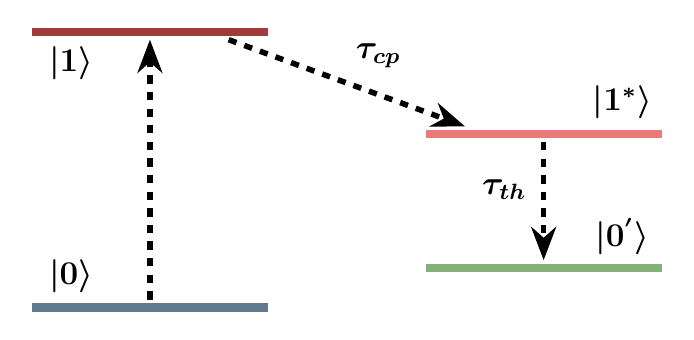
\begin{tikzpicture}
			\draw[cblue, line width=3pt] (0,0) -- (3,0);
			\draw[cred, line width=3pt] (0,3.5) -- (3,3.5);
			\draw[cred2, line width=3pt] (5,2.2) -- (8,2.2);
			\draw[cgreen, line width=3pt] (5,0.5) -- (8,0.5);

			\draw[dashed, -{Stealth}, line width=2pt] (1.5,0.1) -- (1.5,3.4);
			\draw[dashed, -{Stealth}, line width=2pt] (2.5,3.4) -- (5.5,2.3);
			\draw[dashed, -{Stealth}, line width=2pt] (6.5,2.1) -- (6.5,0.6);

			\node at (0.5, 0.4) {\large $\boldsymbol{|0\rangle}$};
			\node at (0.5, 3.1) {\large $\boldsymbol{|1\rangle}$};
			\node at (7.5, 2.6) {\large $\boldsymbol{|1^*\rangle}$};
			\node at (7.5, 0.9) {\large $\boldsymbol{|0^{'}\rangle}$};

			\node at (4.4, 3.2) {\large $\boldsymbol{\tau_{cp}}$};
			\node at (6, 1.5) {\large $\boldsymbol{\tau_{th}}$};
		\end{tikzpicture}
	\end{center}
	\caption{
	Schematic representation of the relaxation pathway following selective
	excitation of hydrogen-bonded O–H vibrations. The initially excited state
	$|1\rangle$ undergoes rapid coupling toward a metastable intermediate state
	$|1^{*}\rangle$ on a characteristic timescale $\tau_{cp}$, corresponding to the
	first energy transfer process. Subsequently, the system relaxes toward the final
	equilibrated state $|0'\rangle$ on a slower timescale $\tau_{th}$, which represent
	the new ground state.}
	\label{fig:HB-trestati}
\end{figure}

% \begin{figure}[t]
% 	\begin{center}
% 		\includegraphics[width=\columnwidth]{figures/HB-trestati.png}
% 	\end{center}
% \end{figure}


The temporal evolution of each modal temperature was analyzed by fitting the data to a bi-exponential model of the form

\begin{equation}
	T(t) = T_{\infty} + A_1 e^{-t/\tau_{cp}} + A_2 e^{-t/\tau_{th}},
\end{equation}

where $T_{\infty}$ denotes the long-time equilibrium temperature, while $\tau_1$
and $\tau_2$ represent the characteristic short and long relaxation times,
respectively. The shorter timescale $\tau_1$ captures the initial coupling process
(intramolecular or intermolecular energy transfer), whereas $\tau_2$ describes
the subsequent thermalization of the considered mode.\\
The relaxation dynamics can be rationalized in terms of a three-state model
involving a metastable intermediate state, as schematically illustrated in
Fig.~\ref{fig:HB-trestati}. Within this picture, $\tau_1$ corresponds to the
population transfer from the initially excited state toward the metastable
configuration, while $\tau_2$ characterizes the slower relaxation toward global
equilibrium.\\
For certain dynamical sectors, the separation between the two timescales is not
clearly resolved within the simulation window. In such cases, a
single-exponential fit was employed and only the dominant relaxation time was
retained.\\

We begin with liquid water. Figure~\ref{fig:vdos_water_a} shows the time-resolved VDOS for excited and non-excited molecules. Immediately after excitation, a pronounced enhancement of spectral intensity appears in the O–H stretching region, confirming the effective population of the targeted vibrational states.
Notably, the initial peak is centered at a slightly lower frequency than the
maximum of the equilibrium stretching band, reflecting the fundamental frequency
of the isolated Lippincott–Schroeder potential used in the Wigner
initialization. As the system evolves, the stretching feature progressively
shifts toward higher frequencies, approaching the equilibrium band position.\\
Concomitantly, a gradual increase of spectral weight is observed in the bending
and low-frequency regions, indicating a redistribution of vibrational energy
toward lower-frequency degrees of freedom.\\
A qualitatively similar spectral evolution is observed in both ice Ih
(Fig.~\ref{fig:vdos_iceIh_b}) and ice IX (Fig.~\ref{fig:vdos_iceIX_c}),
where the initial enhancement in the stretching region is followed by a
progressive redistribution of spectral weight toward lower-frequency modes.
However, compared to liquid water, the spectral features in the crystalline
phases remain sharper, reflecting the more constrained hydrogen-bond network and
increases long-range structural order.\\

\begin{figure*}[p]
	\centering
	\subfloat[]{%
		\includegraphics[width=0.9\textwidth]{figures/water_10perc_temps_all.pdf}
		\label{fig:temps_all_water_a}
	}
	\hfill
	\subfloat[]{%
		\includegraphics[width=0.91\textwidth]{figures/iceIh_10perc_temps_all.pdf}
		\label{fig:temps_all_iceIh_b}
	}
	\hfill
	\subfloat[]{%
		\includegraphics[width=0.9\textwidth]{figures/iceIX_10perc_temps_all.pdf}
		\label{fig:temps_all_iceIX_c}
	}
	\caption{
		Time-resolved modal temperatures and corresponding characteristic coupling times under 10\% vibrational excitation for (a) liquid water, (b) ice Ih, and (c) ice IX.
		Each panel reports the temporal evolution of the modal temperatures associated with O–H stretching, H–O–H bending, librational motion, hydrogen-bond degrees of freedom, and center-of-mass translation, together with exponential fits used to extract relaxation times.
		The inset summary in each panel displays the characteristic intra- and intermolecular coupling times obtained from the fits.
		Across all phases, a clear separation between ultrafast intramolecular relaxation and slower intermolecular thermalization is observed.
	}
	\label{fig:temps_all}
\end{figure*}


While the VDOS provides a clear spectral signature of the excitation, its temporal resolution is inherently limited by the finite window length used in the Fourier transform. In the present case, the 100 fs window implies that spectral estimates are effectively averaged over this timescale, preventing a fully resolved description of faster energy redistribution processes.\\
To overcome this limitation, we analyze the time evolution of modal temperatures, which are defined from the instantaneous kinetic energy projections and therefore provide a frame-resolved characterization of the energy flow between different dynamical sectors.\\
The characteristic coupling times extracted from the bi-exponential fits are
summarized in Fig.~\ref{fig:temps_all}: the time evolution of the modal
temperatures reveals a structured hierarchy of energy redistribution processes.\\

Before discussing said hierarchy, it is useful to isolate the prompt center-of-mass response observed immediately after excitation. In all three phases, the selective initialization of a subset of O–H bonds induces a rapid increase in the center-of-mass kinetic energy of the excited molecules. This feature reflects a direct impulsive
transfer of momentum associated with the non-equilibrium initialization
rather than a genuine thermalization pathway.\\
The timescale of this initial spike depends on the mechanical environment:
it is fastest in ice Ih, intermediate in ice IX, and slowest in liquid
water. In the crystalline phases, the lattice constraints promote a more
direct transfer of the injected momentum to translational motion, whereas
in the liquid phase part of the excess energy is immediately redistributed
among internal vibrational degrees of freedom. For this reason, the prompt
center-of-mass spike is treated separately from the subsequent coupling
processes discussed below.\\

After the initial impulsive response, the energy redistribution enters
an ultrafast intramolecular regime ($t < 100\,\mathrm{fs}$), in which the
characteristic coupling times of librational and bending modes remain
within the same order of magnitude for all phases. Although these
timescales fall within a narrow temporal window ($30–70\,\mathrm{fs}$), their
relative hierarchy is mode dependent. For instance, librational heating
is fastest in liquid water and slowest in ice Ih, whereas the bending
response exhibits a different ordering. This behavior indicates that
the earliest redistribution stage is governed primarily by local
anharmonic couplings, whose efficiency depends sensitively on the
specific vibrational coordinate and on the microscopic structure of
the surrounding hydrogen-bond environment.\\

At intermediate times ($100–500\,\mathrm{fs}$), a clearer differentiation between the
three phases emerges. In this regime, the coupling of unexcited O–H stretching
modes proceeds most rapidly in ice Ih, followed by ice IX, and is slowest
in liquid water. This indicates that the transfer of energy between
stretching coordinates is facilitated in the crystalline environments,
particularly in the proton-disordered phase.\\
In contrast, the redistribution toward unexcited bending degrees of freedom
exhibits a different ordering: liquid water responds most rapidly, followed
by ice IX, while ice Ih displays the slowest heating. The inversion of the
hierarchy between stretching and bending sectors highlights the presence
of competing energy-transfer pathways. Whereas stretch–stretch coupling
appears to benefit from the structural constraints of the lattice,
stretch–bend redistribution is enhanced in the dynamically fluctuating
environment of the liquid phase.\\
This mode-dependent behavior signals a crossover from predominantly local
intramolecular channels to mechanisms increasingly influenced by the
collective structure of the hydrogen-bond network.\\

At longer timescales ($t > 1\,\mathrm{ps}$), the redistribution process becomes
dominated by collective intermolecular motion and global energy transport
through the hydrogen-bond network. In this regime, a systematic hierarchy
between the three phases becomes evident.\\
For hydrogen-bond related motion and center-of-mass degrees of freedom,
liquid water exhibits the fastest approach toward the final equilibrium
temperature, followed by ice IX, while ice Ih displays the slowest
thermalization. This ordering is particularly pronounced in the
center-of-mass relaxation times, where the proton-disordered ice Ih phase
shows significantly longer equilibration times compared to both the
proton-ordered crystal and the liquid.\\
The convergence of librational heating times in the crystalline phases,
together with their marked separation from the liquid case, further
indicates that once energy reaches the collective manifold, its subsequent
redistribution is strongly influenced by the nature of the underlying
network. In liquid water, the presence of continuous structural
rearrangements provides multiple dissipative channels, promoting a
relatively rapid global equilibration. In contrast, the crystalline
phases require energy transport across a more constrained hydrogen-bond
lattice.\\
Within the crystalline systems, the systematically slower thermalization
observed in ice Ih compared to ice IX suggests that proton disorder
introduces additional scattering or mode-mixing effects, reducing the
efficiency of long-range energy transport. In this sense, proton ordering
appears to facilitate a more coherent redistribution of energy through
the hydrogen-bond network.



\section{Conclusions}

\begin{table}[H]
	\begin{ruledtabular}
		\begin{tabular}{l|ccc}
			Mode          & Water    & Ice IX   & Ice Ih    \\
			\colrule
			Libr. exc.    & 0.039266 & 0.053111 & 0.071997  \\
			HOH exc.      & 0.063735 & 0.071081 & 0.049115  \\
			CM exc. spike & 0.095897 & 0.059729 & 0.035687  \\
			OH unexc.     & 0.290093 & 0.216299 & 0.152756  \\
			HOH unexc.    & 0.229555 & 0.279474 & 0.414095  \\
			\hline
			Libr unexc.   & 2.079167 & 0.731097 & 0.753811  \\
			HB            & 2.633747 & 3.621040 & 5.251458  \\
			CM unexc.     & 2.854651 & 3.763624 & 6.053578  \\
			CM exc.       & 4.144040 & 4.401573 & 10.785466 \\
		\end{tabular}
	\end{ruledtabular}
	\caption{}
\end{table}

\clearpage

\bibliography{bibliografia}


\end{document}
